\chapter{Analysis}

\label{analysis}

\subsection{Impact of ICT in homecare}
Existing studies describing the use of ICT in homecare are predominated by positive responses from both chronically ill patients and healthcare professional. As an example, healthcare professional’s opinion is that their work has been facilitated by introducing ICT in homecare. Most studies show that communication between patients and healthcare professional was improved by using ICT. Furthermore, the use of ICT showed cost savings. However, it is important to keep in mind that the use of ICT cannot replace face to face consultations but is an ideal complement \cite{ICT}. It is important to keep in mind that telemedicine supporting already integrated care is associated with the development of new roles within the healthcare system. Ideally, new structures of care delivery at an operational level needs to be supported by corresponding changes at institutional level \cite{countries}. Therefore, by introducing telemedicine both patients and healthcare professional has to be openminded to this new technology and adaptable to change already known working methods. Hence, the development of ICT in homecare should be seen as a learning process and will constantly be evolving and improved based on the ongoing use. 

Another important impact of ICT is the information flow between healthcare professionals. Effective interprofessional communication is highly important within the healthcare system but is seen to be critical when teams are not co-located. For this reason, healthcare professionals who has been in use of an ICT solution pointed out how information via ICT potentially could have and positive effect on patient care and collaboration \cite{barrier}.

Furthermore, exchanging information with patients, follow up and motive them to keep working out and keep having a healthy lifestyle is seen to be easier with ICT. Patients are able to log information, send documents and ask questions more frequently which increases the communication and contact between patient and healthcare professionals. Having more regular discussions with the patient will facilitate more comprehensive and effective collaboration to the patient \cite{barrier}.

\subsection{Implementation of telemedicine in Denmark}
By the European Society of Cardiology, it is a Class I recommendation to follow a cardiac rehabilitation program. This recommendation also includes cardiac patients in Denmark. The effects of a clinical rehabilitation program is clinical approved and there is very strong evidence that it is working. This statement was also mentioned in the interview with Vibeke Lynggaard. Although cardiac rehabilitation is strongly recommended it is seen that long term benefits are often disappointing due to low cardiac rehabilitation uptake and adherence rates. Several studies has been made to indicate the feasibility, safety and effectiveness of cardiac telemedicine rehabilitation. Looking from a cost effectiveness point of view it has been shown that telemedicine rehabilitation is more effective and efficient. Furthermore, is has been concluded that the total cost of an ambulant telemedicine rehabilitation is lower than hospital rehabilitation. A follow up study has shown a reduced number of days lost due to rehospitalization and an increase in days alive and days out of hospital \cite{costeffect, effects}.  

\subsubsection{Rehabilitation offered in Herning Municipality} 

Herning municipality offers free rehabilitation programs for all cardiac patients. The rehabilitation program is known as phase two rehabilitation and consists of a 10-week team progress with 12 patients on every team. The program includes an individual conversation, physical exercise, education and social networking. The team meets twice a week for about two hours and both physiotherapist, nurse and a professional dietary consultant are responsible for the course. At the beginning of the progress the patients are being asked to fill a questionnaire. After respectively 3 and 12 months the patients are being asked to fill the same questionnaire to follow up how the progress is going. 

The purpose of this rehabilitation program is to achieve greater knowledge and understanding of the factors that affect life with a chronic disease. It is important that the patients learn to live life with a chronic disease and how to deal with everyday challenges. Furthermore, it is essential that patients improve physical health, mental fitness and well-being and hereby share experiences with other patients. 

The education will be focusing on better habits within diet, smoking, alcohol and exercise. The physical exercises will consist of different types of training. Both cardio and strength will be included. In corporation with the physiotherapist the right exercise program will be matched to the specific patient in order to physical level and situation \cite{herning}. After participating in phase two rehabilitation patients are offered phase three rehabilitation. This rehabilitation program is based on follow-up and maintenance of treatment, exercise and a healthy lifestyle \cite{Rehabilitering}.

\subsubsection{Outcome}  
It is important to keep in mind that cardiac rehabilitation is a Class I recommendation as has been approved international. Patients are entitled to be offered the best-known rehabilitation program and so far, the centered based rehabilitation is the best rehabilitation program to offer. At the interview with Vibeke Lynggaard she mentioned, that centered based rehabilitation will be hard to replace as it is the best to offer at the moment. An important note from the interview was how telemedicine could be used in phase three rehabilitation. Vibeke Lynggaard mentioned, that all patients are being offered phase three rehabilitation but most of them decides not to participate in the program. This statement indicates, that telemedicine rehabilitation could possibly have an influence and great effect in phase three rehabilitation. This of course rely on the fact that patients decide to participate in the telemedicine solution instead of not participating at all. If more patients agree to participate in phase three rehabilitation where telemedicine is being used, this might have an positive influence on readmission and in the end an cost reducing outcome.  


\subsection{Relative’s Experiences of cardiac Patient’s telemedicine rehabilitation}
It is known that it can be stressful to be a relative to cardiac patients. Most often relatives help with home exercises, medicine dosage and transportation to and from the hospital. They participate in discussions about the patient’s illness and they do housekeeping and practical activities at home, which the patient isn't capable of doing. Research has shown that relatives are in risk of being a patient themselves as a consequence of the stressful job it is to take care of the patient \cite{4, 5}. Therefore, telemedicine rehabilitation is being offered to reduce relative’s homecare. By introducing telemedicine rehabilitation relatives feel more comfortable and secure as the patient is being monitored and healthcare staff react if the patient’s measurements are to be concerned about. By an interview of 13 cardiac patients who participated in telemedicine rehabilitation the results indicated that relatives find telemedicine equipment easy to use and the use of telemedicine motivates the patient to be more active in their own treatment \cite{12}.  

A research has taken place in Denmark where the patient did weekly blood pressure- and weight measurements. A heart rate monitor was used three times a week under physical conditions. Data were shown on an application via smartphone and hereby the patient, relatives and healthcare staff were able to follow the patient’s state of health. For the patients it was a relief that they were able to do exercises and health measurements at home and hereby they were able to do so according to work schedule as well as motivation and mental energy. Furthermore, less hospital visits removes focus on the disease and makes the patient feel more normal and less ill. Hereby patients experience higher quality of life as they feel healthier \cite{Bregendahl_2016}.  

Relatives experienced that everyday life were more normal by using telemedicine rehabilitation as they were able to continue everyday routines and spent less time taking care of the patient. They experienced more freedom as they didn’t have to take the patient to rehabilitation classes, regulate diet and take care of medicine. It indicates that relatives to patients using telemedicine rehabilitation gain more freedom and less concern and responsibility \cite{7}.  

   
\subsection{Comparison with telemedicine solution for COPD patients}

Telemedicine solutions have been tested in pilot projects in different cities in Denmark. The projects have shown that telemedicine can provide financial benefits as well as better and more consistent patients progress and more self-reliant patients \cite{KOL_1}. In 2016 the government, \textit{Kommunernes Landsforening} and Danish Regions did an agreement to offer telemedicine home monitoring to citizens with Chronic obstructive pulmonary disease (COPD) throughout the country by the end of 2019 \cite{KOL_2}. 

In 2014 a pilot project took place in the municipality of Skanderborg were 15 COPD patients were included. After participating in the project, the patients were interviewed to give their perspective on the telemedicine solution. Overall the patients were very satisfied for the solution and especially as they had the freedom to do measurements and exercises whenever they wanted and did not depend on a specific time schedule at the hospital. The only disadvantage the patients were aware of was the connection which sometimes was a bit unstable. For the patients it was very important that picture and sound on the platform was clear and was working optimal at all time, otherwise they lost the motivation. An important observation at this interview was how the patients experiences the social aspect. The patients were used to do exercises at the gym in classes with other patients. Now they had to do exercise at home where they were able to see and talk to each other through the screen. One of the patient’s mentioned that it was a good solution but only for a short time. To him the social aspect was very important, and he didn’t experience the social interaction the same way as he did at the gym. Another important observation was one of the patients who was too ill to get to the hospital and therefore he wasn’t capable of participate at the exercise classes. But by this telemedicine solution he was able to do exercise at home and in the end of the project his physical condition was so good that he was able to do his normal routines at home and also to leave home and go to the hospital. Therefore, this telemedicine solution definitely was an important help to make him feel and get better, Appendix XX.  


\subsection{Challenges within telemedicine rehabilitation} 
\subsubsection{Personal aspect}
The telemedicine solution collides with the GPs’ individual approach, where knowledge on patients’ reaction patterns and personal relationship to the patient is important when assessing the patient and deciding the right intervention. By the use of telemedicine, GPs’ are not able to look at the patient’s overall condition and use knowledge about the patient’s normal reaction. By using telemedicine GPs’ will be looking at measurements measured by the patients themselves and that won’t give the same overall understanding on the patients’ physical condition \cite{Emergence}.  

Furthermore, communication through ICT is seen to be more impersonal and to build up trust to the patient is much more difficult compared to face to face meetings. Visual information such as body language, person interaction and empathy are very important for the therapeutic relationship and this is seen to be a barrier to the effective collaboration between healthcare professional and the patient \cite{barrier}.  

\subsubsection{Funding}

In several countries medical help is funded by health insurance and therefor an ICT solution for a cardiac patient would be financed primarily from the insurance company. This limits the possibility to implement such solutions in foreign countries, as is the health insurance do not want to cover the cost. \cite{considerations}. Denmark in the other hand is primarily funded by the state as explained in \Cref{DHS}. This gives Denmark an unique opportunity to offer the patient the best treatment. In Denmark the municipality takes care of the rehabilitation of cardiac patients. The municipalities receives a fixed amount of money which should be distributed in different areas. If vCare is a cheaper and more sufficient solution it would be worth investing for the municipality. 

An important consideration in funding is the public tendering rules both in Denmark and EU. If a provided service expense, provided by an privat company to a public unit, is more than 1.489.820 DKK the service are ordered to go into public tendering. This process can be expensive for both the company and the public unit. The rules of public tendering is made to secure transparency, equality of treatment, non-discrimination and openness \cite{udbud}. If the ICT service that the municipality wants is less expensive than 1.489.820 DKK the municipality is free to buy the service without going into public tendering. 

\subsubsection{Technological skills}
There are certain technological skills necessary for operating ICT. The majority of cardiac patients are older adults and may not be familiar or comfortable using ICT. Some patients might not be used to use technology on a daily basis and therefore the ICT solution can be a difficult solution for that specific patient group. Additionally, some patients might live in rural areas where adequate internet access is not available. This is seen to be a barrier which has to be considered when introducing ICT \cite{barrier}.  
   
\subsubsection{Ethics}

During the implementation process ethical implications of telemedicine has to be considered to ensure privacy and confidentiality. It is a universal understanding that all patients have rights and healthcare professionals are obliged to respect those rights. When handling patient data, it is important that healthcare professional keep personal information protected. An ethical concern when using telemedicine, it that confidentiality may be more difficult to ensure. To break confidentiality can be seen as breaches of security or inappropriate disclosure of patient data. This kind of inappropriate disclosure applies both videoconferences and viewing electronic medical patient journals \cite{etik}. This big ethical issue is related to the patient's autonomy. It is the patients free right to choose if they want treatment and what treatment they want if multiple treatments is providable. Furthermore, it is the patients right to refuse consent on distributing data or to deny acces on medical records. \\

Edward Chen explains in an article some of the considerations of implementing telemedicine. One of the big concerns is the lack of face-to-face interaction. Telemedicine has a lot of positive effects such as easy patient access, cost reduction, continuative care and a potentially more active patient which can improve compliance, patient satisfaction and anxiety, but it can potentially depersonalize the relationship between healthcare professional and the patient \cite{considerations}.\\ 

Another ethical concern is that every patient should be treated fairly and equitable. People in rural areas should have the same opportunities as people who lives in the city or near the hospitals. The only concern that collides with the use of telemedicine is that the internet connection can be slow in some rural areas and therefore this patient group might experience bad internet acces. This might create som issues though telemedicine mostly gives the patients the same equality hence it will provided in the patients home \cite{considerations}. 

The Danish Healthcare Authority must ensure that patients are offered the best possible treatment. This requires many and high demands to fulfill. Both prevention, diagnostics, treatment and rehabilitation must be carried out with high academic quality and effective utilization of resources. Moreever, it is a requirement that expertise, research, development and education should be continuously expanded and maintained \cite{plan}. With that said it is important to keep in mind that all patients must be offered the best known and evidence based rehabilitation program to ensure that patients are being treated in the best possible way. Therefore, if Herning Municipality decides to introduce telemedicine in rehabilitation it has to be proven that telemedicine rehabilitation is a better and more effective solution than center-based rehabilitation which is used today. Evidens based clinical decisions includes four components: clinical expertise, research evidence, patients' preferences and resources. Clinical expertise and patients preferences may override the two other components as the patients preference will dominate in the treatment decision, although research evidens indicates that another treatment is more preferable for the patient. By using evidens in patient treatment it ensures that the patient are being offered the best treatment based on the best research-based knowledge \cite{evidence}.            


\section{Economy and effect analysis}

The cost part of this analysis will be the implementation cost of standard or telerehabilitation with vCare as the ICT provider. It is important to distinguish between capital expenditure (CAPEX) and Operating expenses (OPEX). For this project the CAPEX to implement standard CR and vCare is collected and the OPEX for running the rehabilitation for the first year. 

\textbf{Comparable basis to randomised controlled trial conducted in Belgium} \label{belgium}

As it wasn’t possible to collect data on cost-effectiveness analysis using QALY and rehospitalization rates, it has been chosen to use data from a previous study. The study that has been used was done in 2015 and carried out in Belgium. The study was made to investigate in the effect of cardiac telerehabilitation in patients with a personalised patient-centred web application. 140 patients suffering from a cardiac disease were randomly allocated to telemedicine rehabilitation (intervention group) or centre-based rehabilitation (control group). Belgium are following the same European CR guidelines as seen in Denmark. Therefore, the rehabilitation program used in the control group is seen to be the same as the one used in Herning Municipality. The study period for the control group was three month and the group participated in group-based training sessions at the rehabilitation centre. The group size varied from 8-12 patients per session and they were under supervision of physical therapist and exercise specialist, both specialised in CR. The rehabilitation program started with an individual physical test on an electromagnetically braked cycle ergometer. In the end of the program the patient’s physical health were evaluated by a nurse. Furthermore, the CR programme consisted of an information / education module, smoking cessation and dietician guidelines \cite{costeffect}. 

As seen in the below section the study conducted in Belgium can be compared to the 12-weeks rehabilitation program used in Herning. Therefore, QALY and rehospitalization rates are evaluated as useful data to be used in this project. \\


The Economic analysis in this paper does not include a detailed analyse of phase 1 which is the period of hospitalization of the patient. This is dismissed because the cost of the control group and intervention group is the same in this phase of rehabilitation. Furthermore, the introduction of tele rehabilitation will not affect this phase of rehabilitation. Moreover, phase three will not be included in this analysis because lack of knowledge on cost in this specific phase. However,  telemedicine could possibly have a great effect on phase three rehabilitation.  

Phase 2 is the phase after the patient has been discharged and this is the phase that will be included in this analysis.


\subsection{Control group}

The control group in this cost-effectiveness analysis is as before mentioned the standard CR in Herning Municipality. The  patients in the control group participates in a 12 week session within the municipalities training facility. 200 patients are on average in the program yearly.

\subsubsection{Economics}
Almost all cost for the control group was collected during the semi-structured interview with Eva Klose Jensen and Hanne Voldgaard Nielsen described in \Cref{sec: evahanne}. If a cost has been collected elsewhere it will be described throughout this section. 

The cost of profession is the first cost that is taken into account.
The salary and working hours of the professions needed in the control group is based on the cost in Herning Municipality. This means that the cost on this element will differ from municipality too municipality as the salary may vary.  The collected data will be described further in this section where cost per patient will be the outcome of the calculations. 


The salary of the nurses needed in the standard CR is 308DKK per hour and they have two nurses who works 21 hours, 48 weeks a year. The cost per patient will therefore be as follows:

Total hours of working nurses a year:

$$42hours\cdot48weeks=2016hours$$

Total cost per year:
$$2016hours\cdot308DKK=620.928DKK$$

Cost per patient:
$$\frac{620.928DKK}{200patients}=3104,64DKK$$

The cost per year for the physiotherapist is 600.000DKK hence the calculations for the physiotherapist is backwards. The physiotherapist works 54 hours a week in 48 weeks a year. The cost of the physiotherapist is therefore as follows:

Total hours of working physiotherapist a year:
$$54hours\cdot48weeks=2592hours$$

Physiotherapist hourly cost:

$$\frac{600.000DKK}{2592hours}=231,50DKK$$

Cost per patient:
$$\frac{600.000DKK}{200patients}=3000DKK$$

The salary of the dietician needed in the standard CR is 225DKK per hour. The dietician is schedule to participate four times a year for three hours. Furthermore, the dietician get paid for two hours of preparation per class. Therefore, the cost of the dietician is as follows:

Total hours of working dietician a year:

$$5hours\cdot4=20hours$$

Total cost per year:
$$20hours\cdot225DKK=4500DKK$$

Cost per patient:
$$\frac{4500DKK}{200patients}=22,5DKK$$

\begin{table}[H]
\begin{longtabu} to \linewidth{@{}l l l X[j]@{}}
    \textbf{Profession} & \textbf{Average hourly Cost} & \textbf{Total cost a year} & \textbf{Cost per patient} \\[-1ex]
    \midrule
     Nurse   &    308 DKK & 620.928DKK & 3104,64DKK \\ \hline
    Physiotherapist   &   231,50DKK  & 600.000DKK & 3000DKK \\ \hline
    Dietician   &  225DKK &    4500 DKK    & 22.5DKK \\ \hline
    Technician & 200DKK & 0DKK & 0DKK\\
    \hline \hline \hline
    \textbf{Total} & & 1.225.428DKK & 6127,14DKK
    \newline
   \end{longtabu}
\caption{Profession control group cost}
\label{tab: PC}
\end{table}

The next cost that is considered is the implementation cost of materials such as training equipment and office supplies at the training facility. It is important to notice that these costs is a one-time cost and therefore it will be a significant minor cost in the future. The data is collected from a spreadsheet handed out from Herning Municipality. To see the spreadsheet with exact prices on all materials please see Appendix XXXX.

\begin{table}[H]
\begin{longtabu} to \linewidth{l l l l }
    \textbf{Materials implementation} & \textbf{Unit} &\textbf{Total Cost} & \textbf{Cost per patient} \\[-1ex]
    \midrule
    Training equipment   &  97 &  29.711DKK & 149DKK \\ \hline
    Training bikes   & 12 & 118.200DKK & 591DKK  \\ \hline
    Test bike    &  1 & 76.750DKK &   382.75DKK \\ \hline 
    Office supplies    &  39 & 34.545DKK  &   173DKK  \\ \hline 
    Other material   &  8 & 18.161DKK  &   91DKK\\
    \hline \hline \hline
    \textbf{Total} & 157 & 277.367DKK & 1386,75DKK
    \newline
   \end{longtabu}
\caption{Materials control group cost}
\label{tab: MC}
\end{table}

To provide the right and most effective care for the patient and to follow up on their medical condition, some medical equipment is needed. These are described in \Cref{tab: MeC}. This data is based on the spreadsheet as before mentioned and is to be seen in Appendix XXX.

\begin{table}[H]
\begin{longtabu} to \linewidth{l l l l}
    \textbf{Medical equipment} & \textbf{Unit} &\textbf{Total Cost} & \textbf{Cost per patient} \\[-1ex]
    \midrule
    Model of heart   &  1 &  350DKK & 1,75DKK \\ \hline
    Sphygmomanometer  & 1 & 1599DKK & 8DKK  \\ \hline
    Pulse Oximeter    &  1 & 599DKK &   3DKK \\ \hline 
    Cuff    &  2 & 498DKK  &   2,5DKK  \\ \hline 
    Ventilation mask   &  1 & 1637DKK  &   8DKK \\
    \hline \hline \hline
    \textbf{Total} & 6 & 4683DKK & 23,25DKK
    \newline
    \newline
   \end{longtabu}
\caption{Medical equipment control group cost}
\label{tab: MeC}
\end{table}

The rest of the costs in Herning Municipality is collected in \Cref{tab: OC}. The cost for renting the facility is not given in the table. This is due to a non-disclosure agreement with Herning Municipality. The group is aware that this specific value is a big part of the overall cost. Unfortunately, is it not possible to publish the number in this paper. 

The number of re hospitalized patients in Region Midtjylland was 4658 in 2015 out of 20289 admissions, hence the percentage of rehospitalization per patient is 23\% in the Region. Keep in mind that some patients are re hospitalized twice and therefore the total number of readmissions is 6339, which means a total percentage of 31\% readmissions \cite{hjertetal}. It is not possible to collect the exact data from Herning Municipality. The total cost is calculated as it is expected that 23\% of all patients in CR treatment in Herning Municipality in re hospitalized. The average cost of rehospitalization was 100.875DKK in 2004 \cite{rasmussen2011hjerterehabilitering}. This is the newest number that has been collected, but the cost is higher today, but unknown. The calculation of cost in Herning Municipality is as followed.

Estimated number of readmissions to Herning Hospital:


$$31\%200= 62 readmission$$

Total cost:
$$62\cdot100.875DKK=6.254.250DKK$$

Total cost spread out as a cost on all patients:

$$\frac{6.254.250DKK}{200}=31.271,25DKK$$

\begin{table}[H]
\begin{longtabu} to \linewidth{l l l l }
    \textbf{IT} & \textbf{Unit/ hourly cost} &\textbf{Total Cost} & \textbf{Cost per patient} \\[-1ex]
    \midrule
    IT license  & 0  & 0DKK  & 0DKK  \\  \hline
    IT training & 0 & 0DKK & 0DKK \\
    \hline \hline \hline
    \textbf{Total} &  &  & 
    \newline
    \newline
   \end{longtabu}
\caption{IT equipment control group cost}
\label{tab: ITC}
\end{table}

\begin{table}[H]
\begin{longtabu} to \linewidth{@{}l l l X[j]@{}}
    \textbf{Other Cost} &\textbf{Total Cost a year} & \textbf{Cost per patient} \\[-1ex]
    \midrule
    Location   &  (NDA) & (NDA) \\ \hline
    Employee education   & 10.000DKK & 50DKK  \\ \hline
    HjerteKomMidt (database)  & 34.346 DKK &   171,75DKK \\ \hline
    Brochure & 0DKK & 0DKK \\ \hline
    Rehospitalization & 6.254.250DKK & 31.271,25DKK \\
    \hline \hline \hline
    \textbf{Total} & 6.298.596DKK  & 31.493DKK
    \newline
    \newline
   \end{longtabu}
\caption{Other cost control group}
\label{tab: OC}
\end{table}


From these collected costs from Herning Municipality it is possible to calculate the total cost and total cost per patient after the first year of implementation. This total cost includes both CAPEX and OPEX.

Total cost for implementation and first operational year:
$$1.225.428 + 277.367 + 4683 + 6.298.596 = 7.806.074DKK$$

Total cost per patient for implementation and first operational year:

$$6127,14+1386,75+23,25+31.493= 39.030DKK$$


\subsubsection{Effectiveness}

 The Adjusted mean QALY in the control group is 0.36 and this is the number that will be used in the cost-effectiveness analysis in this paper\cite{costeffect}. 

\subsection{Intervention group}

The intervention group are following a 12-week rehabilitation program as the control group. Based on the number of 200 patients in the standard CR in Herning Municipality the calculation in this section is based on a maximum of 50 patients attending a program at the same time. This will give a maximum 200 patients follow the program on a yearly basis. 

\subsubsection{The silver package}

The composition of the silver package is based on the knowledge of the existing CR equipment and minimized hours of health professionals. Both CAPEX and OPEX is a part of the setup which makes it comparable to the control group. 

The patients using the silver package will be tested before starting the treatment and in the end of the treatment and for this test some tools are needed. In this case the same equipment is taken into account as what is used in the standard CR in Herning Municipality. Added to this is the IT-equipment which in this case is a tablet and a license for using the rehabilitation program. The program will consist of a virtual trainer, dieting advises, materials focusing on the illness and other knowledge on health risk. The training equipment in this package is the minimum amount of equipment used in a training setup, it is estimated that the combination of weights, yoga mats, step benches and a training bike is suitable constitution. By this few training components it has been estimated that it is possible to perform an exercise program similar to the one that is being used in the centre-based rehabilitation program in Herning Municipality. 

The composition of health professionals is an estimation based on a minimum need.  First of all, the need of testing patients medical condition before and after the program is still important. Furthermore, it is important to create an individual program for each patient hence three hours of nurse and physiotherapist are provided to take care of both the testing and creation of the individual program. Moreover, one hour of providing suitable diets for the patient made by a dietician is set in the program.
 
Throughout the program it is possible to be checked up on by a nurse for this matter one-hour per patient is provided. 

There is a need of a technician to set up the IT and perhaps the training equipment in the patients home. Furthermore, if there is some trouble with the technology during the program and technician is available for IT support. For this matter two hours of help from a technician is provided. Last but not least the patient is in need of some training on how to use the application and to do so one hour of instruction is provided. 

The other costs in the intervention group is quite similar to the control group because most of the expenses is mandatory for the municipality. The only cost that changes is the rehospitalization as this number is based on study in Belgium \cite{costeffect} which will be further described in the section of the table, \Cref{tab: OI}. 

\subsubsection{Economics}

The nurse hours are calculated as one even though some hours are used for testing the patient before and after the cardiac tele rehabilitation and other hours will be spend during the 12 week training period. Three hours have been included on testing the patient and creating the best fitted solution for the individual patient.

Total hours of working nurse per patient:
$$1hour + 3hours=4hours$$

Total hours of working nurses per 200 patients:
$$4hours + 200patients=800hours$$

Total cost per year for 200 patients:
$$800hours\cdot308DKK= 246.400DKK$$

Cost per patient:
$$4hours \cdot 308DKK=1232DKK$$

The physiotherapist is in the same setup as the nurse and the calculations are as followed.

Total hours of physiotherapist per patient:
$$1hour + 3hours=4hours$$

Total hours of working nurses per 200 patients:
$$4hours + 200patients=800hours$$

Total cost per year for 200 patients:
$$800hours\cdot231,50DKK= 185.000DKK$$

Cost per patient:
$$4hours \cdot 231,50DKK=926DKK$$

The dietician is included to personalize a diet for the patient, the hours is mostly in the start of the program but within the hour it will be possible to reevaluate the diet during the rehabilitation.  

Total hours of working dietician per 200 patients:

$$1hours\cdot200patients=200hours$$

Total cost per year:
$$200hours\cdot225DKK=45.000DKK$$

Cost per patient:
$$\frac{45.000DKK}{200patients}=225DKK$$

The technician is working two hours per patient and is provided with a wage of 200DKK. 
Total cost per year:
$$400hours\cdot200DKK=40.000DKK$$

Cost per patient:
$$\frac{40.000DKK}{200patients}=400DKK$$

\Cref{tab: PI} shows the estimated cost of professions when implementing the silver package and the operation cost for the first year.

\begin{table}[H]
\begin{longtabu} to \linewidth{@{}l l l X[j]@{}}
    \textbf{Profession} & \textbf{Average hourly Cost} & \textbf{Total cost a year} & \textbf{Cost per patient} \\[-1ex]
    \midrule
     Nurse   &    308 DKK & 246.400DKK & 1232DKK \\ \hline
    Physiotherapist   &   231,50DKK  & 185.200DKK & 926DKK \\ \hline
    Dietician   &  225DKK &    45.000 DKK    & 225DKK \\ \hline
    Technician & 200DKK & 80.000DKK & 400DKK \\
    \hline \hline \hline
    \textbf{Total} & & 556.600DKK & 2.783DKK
    \newline
   \end{longtabu}
\caption{Profession Intervention group cost}
\label{tab: PI}
\end{table}

In \Cref{tab: MI} the materials and medical equipment expenses is shown for implementing rehabilitation in a patients home and test facility in the municipality. The units vary depending on whether it should be in every patients home or only used in the test of the patient. The prices on the training materials is the same provider as Herning municipality used when they implemented their rehabilitation unit in 2017.

\begin{table}[H]
\begin{longtabu} to \linewidth{@{}l l l l X[j]@{}}
    \textbf{Materials implementation} & \textbf{Unit} & \textbf{Cost per unit}&\textbf{Total Cost} & \textbf{Cost per patient} \\[-1ex]
    \midrule
    Training weights   &  $4\cdot50$ & 200DKK&  40.000DKK & 200DKK \\ \hline
    Test bike   & 1 & 76.750DKK & 76.750DKK & 384DKK  \\ \hline
    Training bike & 50 & 9850KK& 492.500DKK & 2462,50DKK \\ \hline
    Yoga mat   &  50 & 99DKK& 4950DKK &   24,75DKK \\ \hline 
    Step bench    &  50 & 399DKK & 19.950DKK  &   99,75DKK  \\ \hline 
    Tablets   &  50 & 2790DKK& 139.500DKK  &   697,50DKK\\ 
    \hline \hline \hline
    \textbf{Total} & 401 &  & 773.650DKK & 3868,50DKK
    \newline
   \end{longtabu}
\caption{Materials intervention group cost}
\label{tab: MI}
\end{table}

\begin{table}[H]
\begin{longtabu} to \linewidth{l l l l }
    \textbf{Medical equipment} & \textbf{Unit} &\textbf{Total Cost} & \textbf{Cost per patient} \\[-1ex]
    \midrule
    Sphygmomanometer  & 1  &1599DKK & 8DKK  \\ \hline
    Pulse Oximeter    &  1 & 599DKK &   3DKK \\ \hline 
    Cuff    &  2 & 498DKK  & 2,5DKK  \\ \hline 
    Ventilation mask   &  1 & 1637DKK  &   8DKK \\
    \hline \hline \hline
    \textbf{Total} & 5 & 4333DKK & 21,50DKK
    \newline
    \newline
   \end{longtabu}
\caption{Medical equipment Intervention group cost}
\label{tab: MeI}
\end{table}

The IT license is based on a expert estimation of the monthly price for such ICT solution \cite{sofoklis}. 
The expenses related to IT is shown in \cref{tab: II}.

\begin{table}[H]
\begin{longtabu} to \linewidth{l l l l }
    \textbf{IT} & \textbf{Unit/ hourly cost} &\textbf{Total Cost} & \textbf{Cost per patient} \\[-1ex]
    \midrule
    IT license  & 3  & 27.000DKK  & 135DKK  \\ \hline
    IT training & 200DKK & 40.000DKK & 200DKK \\
    \hline \hline \hline
    \textbf{Total} &  & 67.000DKK & 335DKK
    \newline
    \newline
   \end{longtabu}
\caption{IT equipment Intervention group cost}
\label{tab: II}
\end{table}

The costs of rehospitalization are based on the same numbers as used for the control group\cite{hjertetal, rasmussen2011hjerterehabilitering}. The percentages of rehospitalization are quite hard to estimate and therefore the results from the study in Belgium is included in this calculation. The percentage of rehospitalization in the intervention group in Belgium was 17\% \cite{costeffect}.

Estimated number of readmissions in Herning Hospital:


$$17\%200= 34 readmission$$

Total cost:
$$34\cdot100.875DKK=3.429.750DKK$$

Total cost spread out as a cost on all patients:

$$\frac{3.429.750DKK}{200}=17.3505DKK$$

\begin{table}[H]
\begin{longtabu} to \linewidth{@{}l l l X[j]@{}}
    \textbf{Other Cost} &\textbf{Total Cost} & \textbf{Cost per patient} \\[-1ex]
    \midrule
    Location   &  0 & 0 \\ \hline
    Employee education   & 10.000DKK & 50DKK  \\ \hline
    HjerteKomMidt (database) & 34.346 DKK &   171,75DKK \\ \hline
    Brochure & 0DKK & 0DKK \\ \hline
    Rehospitalization & 3.429.750 & 17.148,75DKK \\
    \hline \hline \hline
    \textbf{Total} & 3.474.096DKK  & 17.370,50DKK
    \newline
    \newline
   \end{longtabu}
\caption{Other cost Intervention group }
\label{tab: OI}
\end{table}

From these self-estimated and collected costs from Herning Municipality it is possible to calculate the total cost and total cost per patient after the first year of implementation the silver package in Herning Municipality. This total cost includes both CAPEX and OPEX cost.

Total cost for implementation and first operational year:
$$556.600 + 773.650 + 4333 + 67.000 + 3.474.096 = 4.875.676DKK$$

Total cost per patient for implementation and first operational year:

$$2.783+3868,50+21,50+335+17.370,50= 24.378,50DKK$$

\subsubsection{Effectiveness}

The Adjusted mean QALY in the intervention group is 0.39 and this is the number that will be used in the cost-effectiveness analysis in this paper\cite{costeffect}. 

\subsection{Results}

The cost and effectiveness obtained in the previous sections is used to calculate the Incremental Cost-Effectiveness Ratio which will elaborate on whether the solution is cheaper or more expensive due to effectiveness compared to the center-based rehabilitation program.  

$$ICER = \frac{Cost \quad I - Cost \quad C(DKK)}{Effectiveness \quad I - Effectiveness \quad C(QALY)}$$ 

$$\frac{24.378,50-39.030(DKK)}{0.39-0.36(QALYs)}=-488.383,33(DKK/QALY)$$ 

This Incremental Cost-effectiveness ratio indicates that -488.383,33DKK would be saved per gained QALY when exchanging standard CR with telemedicine. 

A scatterplot can be used to visualize the cost effectiveness. \Cref{fig:scatter} is the scatterplot from the study in Belgium \cite{costeffect}. The results in this analysis will be placed in the fourth quadrant as well as the results from Belgium. The scatter plots tell that QALY is increased and the cost is declining when introducing an ICT solution in CR.  


\begin{figure}[H]
\centering
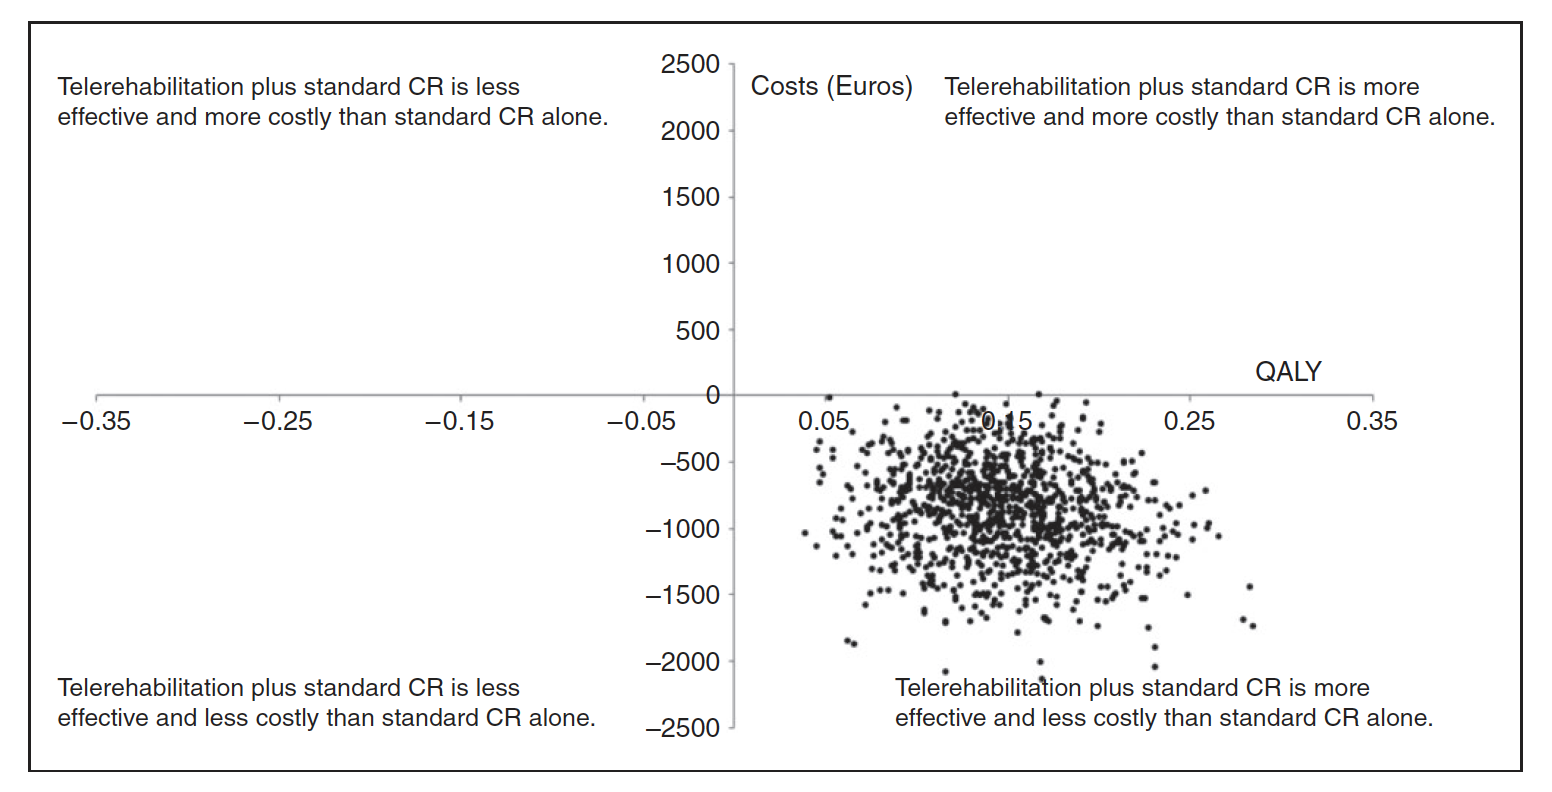
\includegraphics[width=1\textwidth]{Figure/scatter.png}
\caption{Scatterplot from comparable study \cite{costeffect}}
\label{fig:scatter}
\end{figure} 

\chapter{Discussion}

\textbf{A rehabilitation solution with respect to the patients needs} \newline
Cardiac rehabilitation has proven beneficial effects on morbidity and mortality and is highly recommended by international guidelines within the European Society of Cardiology \cite{ESC}. These guidelines contain evidence exists for selected items to be offered in cardiac rehabilitation and therefore it can be a difficult task to replace the centre-based rehabilitation program which is used internationally today. Unfortunately, CR is underutilised due to patient related factors such as traveling distance, social aspects and/or work schedule. As reported in a randomized controlled trial in Herning Municipality \cite{rehab}, only 50\% of the patients who are being offered to follow a rehabilitation program accepts the offer. Furthermore, it is seen that improvements on lifestyle behaviour, such as physical condition and nutrition, are often not maintained over time \cite{CAD}. This statement was also concluded in the patient interview, \Cref{patientinterview}, where a nurse mentioned that three years after participating in the rehabilitation program most patients are back to the same state of health as they were before participating in the rehabilitation program. With these aspects in mind telemedicine rehabilitation can possible be a beneficial solution to be offered as part of the centre-based rehabilitation program. To accommodate the patients’ needs a telemedicine solution would be beneficial after the 12-weeks of centre-based rehabilitation. By this solution patients could possible continue on both exercises and nutrition programs made by physiotherapist and dietitian. This solution could possibly be implemented as an application that can be downloaded to both smartphones and tablets. The application could consist of exercise programs with different levels to accommodate patients with different physical shape. Also, nutrition programs made with regard to cardiac patients could be included. Furthermore, information and knowledge within heart disease, risk factors, medicine, etc. could be a part of the application. This solution would not be used to reduce exact cost on the rehabilitation program that is being used today. It could possible help patients after the rehabilitation program and hereby is could possibly be cost effective due to readmission as hopefully patients would stay in good physical shape. 


\subsection{Implementation}

\subsubsection{Legislation} 
Due to the new EU Legislation \textit{The General Data Protection Regulation} (GDPR), which will take effect on the 25 of May 2018, protection of personal data is at high relevance at the moment. A new regulation was necessary to take into a account and the changes was mostly trigged by an increased use of internet in healthcare and new technologies such as telemedicine \cite{GDPR}. Telemedicine generates huge amounts of data, including both health data but also location- and movement data is identified. GDPR will provide a secure use of telemedicine services both with respect to collection, processing and storage of personal data. New provisions around anonymisation of personal data and the right to be forgotten are intended to drive trust and hopefully break down some barriers, due til secure data management, in the implementation process of telemedicine. Furthermore, the regulation will provide a more harmonised regulatory framework for all telemedicine service providers.   

\subsubsection{BIAS}

Interviews 

udregninger: kommer fra et andet studie - modellen er anderkendt


%diskuter resultat for økonomi, med henblik på at fjerne udgift til re hospitalisering og se om det stadig er billigere 

%BIAS + kilde kritik


% Vi skal skrive noget om at telemedicine ikke kun skal være cost beneficial men også effective and good for the patient. 

%metode

% vi skal være meget opmærksomme på bias i vores diskussion af data collection brug KAspers bog til sætte de korrekte ord på. 




%Nedstående kan anvendes som argumentation
 %"These programs are only successful, though, if patients take initiative in the self-management of their chronic diseases. Furthermore, once equipment is installed, extensive patient or caregiver education is required in order to properly use these devices and obtain accurate measurements. Once the data is transmitted daily to the control center in the hospital, a nurse reviews the data for any alerts, notifying the patient’s provider for follow-up if these results are not consistent with that patient’s usual state of health. The benefits of home health telemedicine, or telehealth, include improved compliance, improved patient and caregiver satisfaction, decreased anxiety, increased quality of life, and patient empowerment through active participation in managing their own diseases. From a healthcare professional perspective, telehealth offers daily monitoring and management, preventative care, early intervention, improved provider-patient communication. Furthermore, it creates efficiencies and cost savings by allowing providers to manage and monitor multiple patients simultaneously, which reduces ER visits and improves allocation of scarce medical resources." \cite{considerations}.
 
 % Nedstående er mulige ting der kan anvendes forskellige steder i rapporten
 %"The patients' self-monitoring of the disease should be enhanced and technologies for self-monitoring should be evaluated and the quality of the monitoring should be assured."\cite{NationalBoardofHealth}

\chapter{Recommendation}

\chapter{Perspectivation}
%Kan også være refleksion

\subsection{Ongoing project in Netherlands}

A project in Netherlands is looking into the impact of ICT solution for a group of cardiac patients. The patient group has been diagnosed with coronary artery disease (CAD). The result of the trial it not yet submitted as the trial is ongoing. The study is looking into 300 patients whereas 150 are restricted as a control group. The control group will receive normal Cardiac Rehabilitation (CR) treatment and the intervention group will receive home-based telemedicine rehabilitation\cite{CAD}. 
The result of this study could have a great impact on this project.

\subsection{Future work}
% Her skal komme noget om fælles udbud telemedicin


%Future work what would it cose to develop(note fra sofoklis)











